\documentclass[a4paper]{article}
\usepackage{latexsym,amssymb,amsmath,amsbsy,amsopn,amstext,xcolor,multicol}
\usepackage{ctex,hyperref,graphicx,wrapfig,fancybox,listings,subfigure}
\usepackage{pgf,pgfarrows,pgfnodes,pgfautomata,pgfheaps,pgfshade,tikz}
\usepackage[top=1in, bottom=1in, left=1.25in, right=1.25in]{geometry}
\graphicspath{{pic/},{draughts-server/}}
\title{
\includegraphics[scale=0.1]{icon_xl.png} \bf Draughts Game}
\date{2017.9}
\author{计64~~翁家翌~~2016011446}
\begin{document}
\kaishu
\ttfamily
\maketitle
%\tableofcontents
%\newpage
\section{软件用途}
本软件是一个国际跳棋小游戏,使用Qt5编写,实现了国际跳棋游戏的双人网络对战版,以及任意局面的输入功能。
\section{运行方式}
安装Qtcreater之后,将源代码拷贝至本机,源代码位于\url{https://git.thusaac.org/trinkle/draughts-qt5}。运行Qtcreater直接编译即可。

经过测试,Ubuntu和Mac运行良好,Windows系统下可能会崩溃,真心玄学……
\section{功能介绍}
\subsection{游戏界面}

\begin{figure}[htp]
\centering
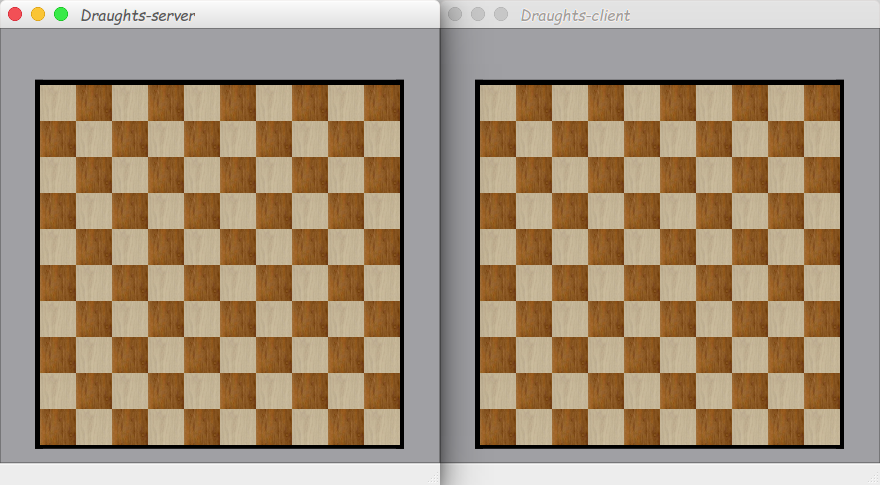
\includegraphics[width=1\linewidth]{init.png}
\caption{开始界面}
\label{fig:start}
\end{figure}

图~\ref{fig:start} 显示了软件的开始游戏界面。最上方为选项栏,中部是棋盘界面,在棋盘上面会显示黑白双方的剩余子力,最下面的状态栏会显示连接到的IP地址和端口信息。

游戏界面支持任意比例放缩。

\subsection{选项栏}
\begin{figure}[htp]
\centering
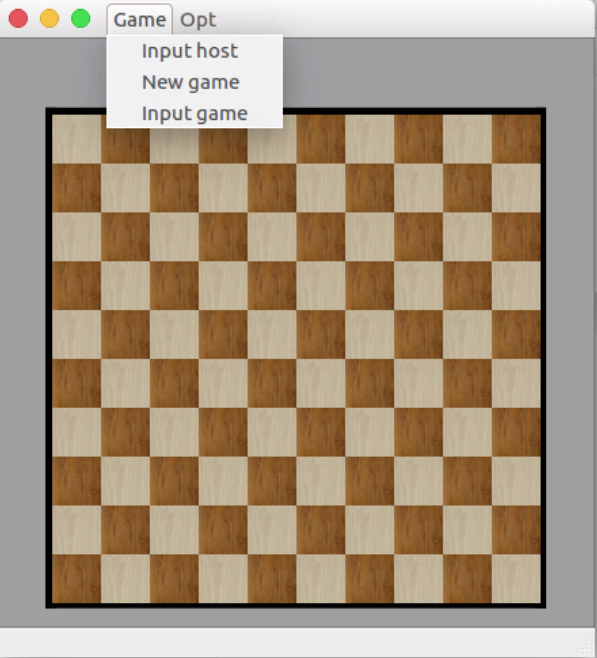
\includegraphics[width=0.5\linewidth]{game.png}
\caption{标题选项栏(Server)}
\label{fig:title}
\end{figure}

图~\ref{fig:title} 显示了软件主机端的标题选项栏。在\uline{G}ame选项下有三个子选项,分别是\uline{Input host}、\uline{New game}和\uline{Input game}。当且仅当Input host成功并且连接客户端成功之后,其他选项才能正确运行。在\uline{O}pt选项下有两个子选项,分别是\uline{Make a draw}和\uline{Give up}。点击相应的选项之后,会向另一方发送请求。

客户端的标题选项栏与主机端有一定区别,在\uline{G}ame选项下只有\uline{Input host}选项,也就是说游戏界面的控制权处于主机端。

\subsection{连接界面}
\begin{figure}[htp]
\centering
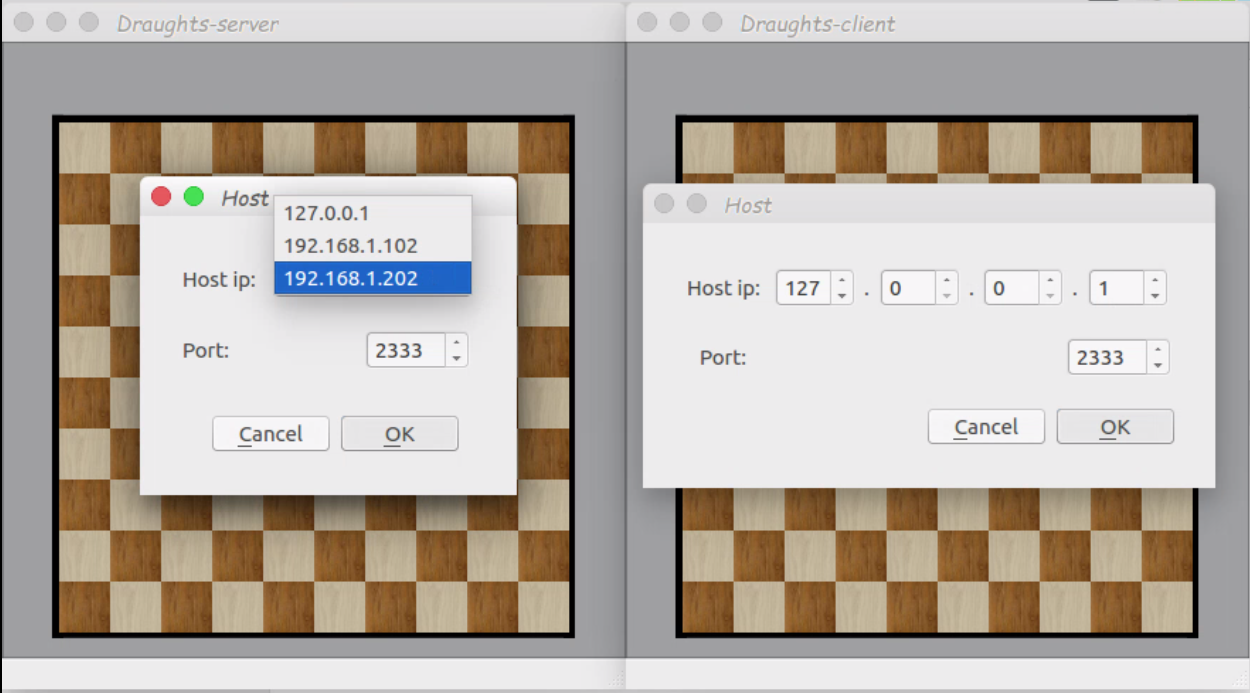
\includegraphics[width=0.8\linewidth]{host.png}
\caption{连接界面选项卡}
\label{fig:host}
\end{figure}

\begin{figure}[htp]
\centering
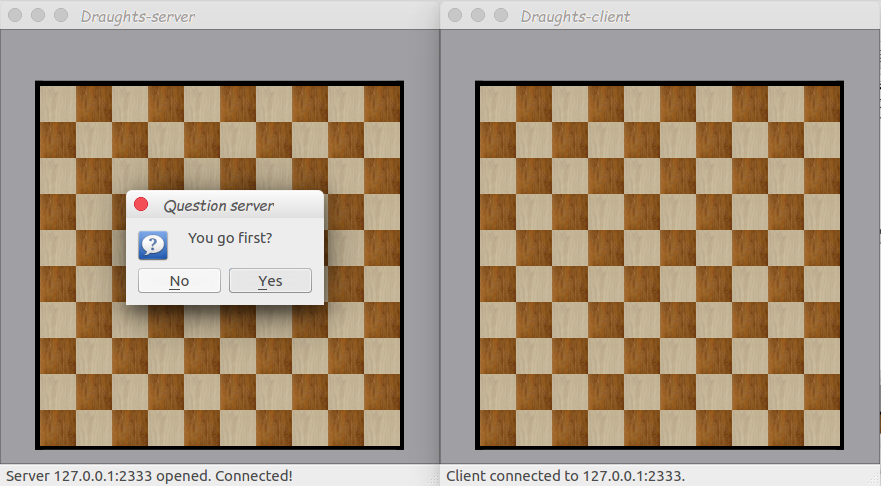
\includegraphics[width=0.8\linewidth]{go.png}
\caption{连接成功界面}
\label{fig:go}
\end{figure}


图~\ref{fig:host} 显示了主机端和客户端的连接界面。在主机端(左侧)中,程序会自动检测本机的所有能够使用的IP地址并在选项卡中显示,端口号能够自定义。在客户端(右侧)中,可以手动输入IP地址和端口号进行连接。

图~\ref{fig:go} 显示了连接成功之后的界面。当连接成功之后,双方界面最下方会显示连接的IP,并且在主机端会弹出选项卡,询问是否先手(先手执黑,后手执白)。当主机端确认之后,双方游戏开始。

\subsection{自定义棋局}
\begin{figure}[htp]
\centering
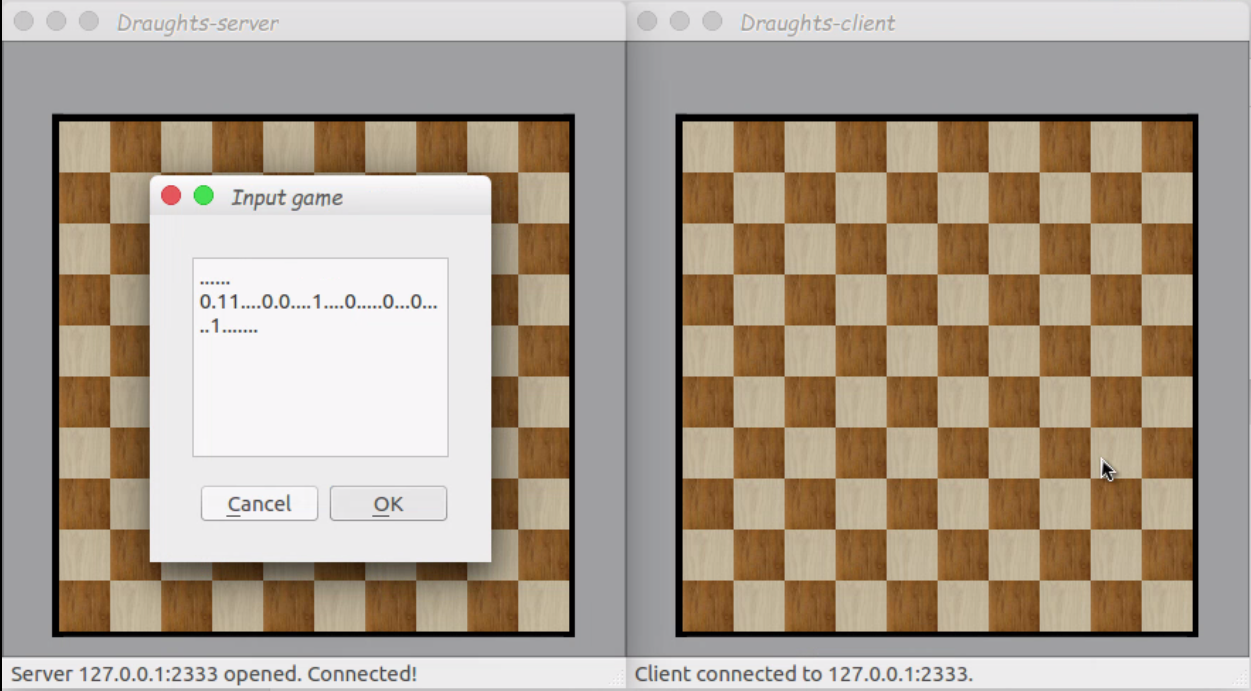
\includegraphics[width=1\linewidth]{input.png}
\caption{自定义棋局}
\label{fig:custom}
\end{figure}

图~\ref{fig:custom} 显示了主机端在点击\uline{Input game}之后弹出的对话框,用户可以在对话框内输入任意棋局,共50个字符,每行从左到右依次输入,"\uline{.}"表示空格,"\uline{0}"表示白兵,"\uline{1}"表示黑兵,"\uline{2}"表示白王,"\uline{3}"表示黑王。点击 \fbox{OK} 按钮之后即可开始游戏。

\subsection{游戏界面}
\begin{figure}[htp]
\centering
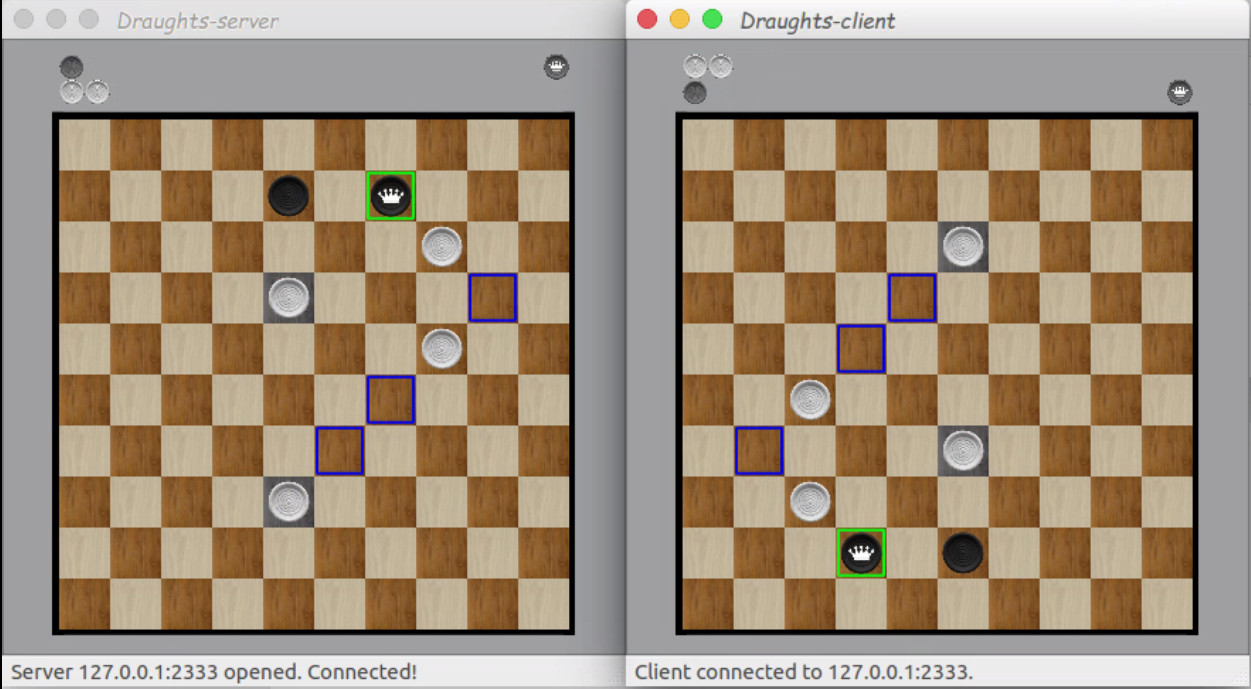
\includegraphics[width=1\linewidth]{state.png}
\caption{运行界面}
\label{fig:status}
\end{figure}

图~\ref{fig:status} 显示了软件在游戏过程中的运行界面。在一方使用鼠标点击的时候,另一方会实时看到对方的点击动作。在鼠标未点击的时候,程序会用绿色方框框出能够被选中的棋子;在鼠标点击了一个能够被选中的棋子之后,程序会用蓝色方框框出这个棋子能够经过的路径;被吃掉的棋子的背景会变为灰色。

在棋盘上方会实时显示双方的棋子数目,左侧为普通棋子,右侧为王,第一行为对方棋子,第二行为自己棋子。图~\ref{fig:status} 中,Server(左侧)执白,Client(右侧)执黑。

\begin{figure}[htp]
\centering
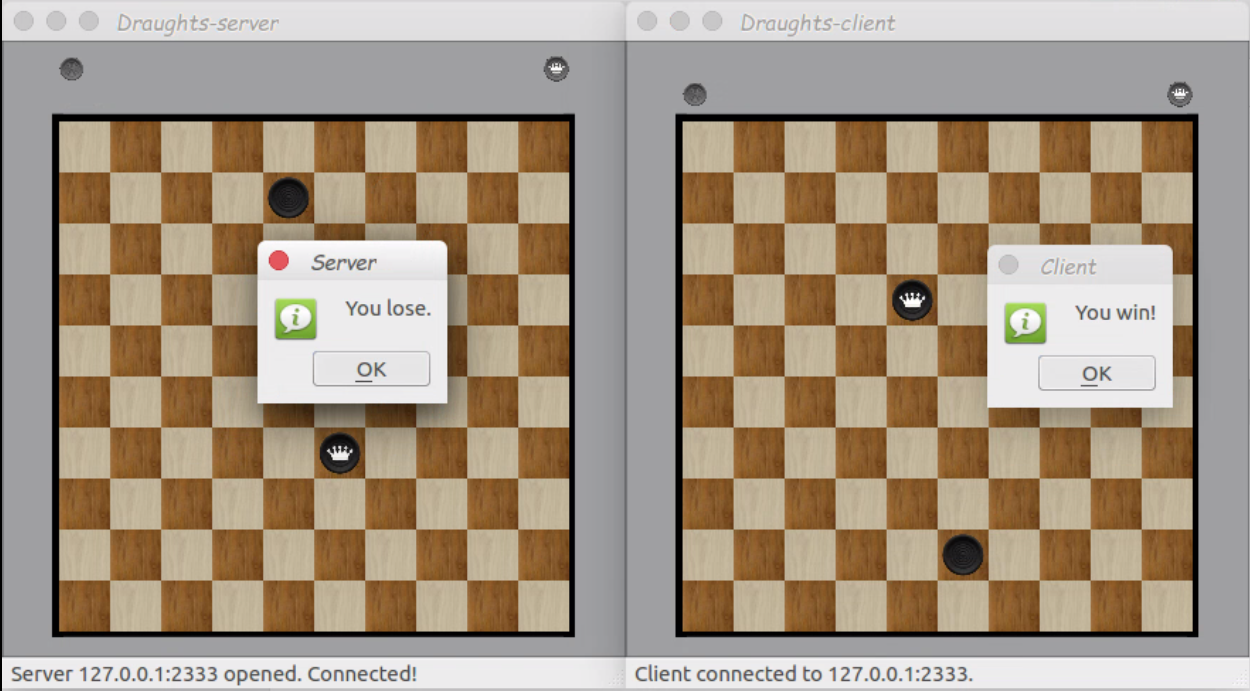
\includegraphics[width=1\linewidth]{finish.png}
\caption{游戏结束}
\label{fig:finish}
\end{figure}

图~\ref{fig:finish} 显示了软件在游戏结束时候的界面。双方均会弹出输赢的对话框。

\subsection{认输及求和}

\begin{figure}[htp]
\centering
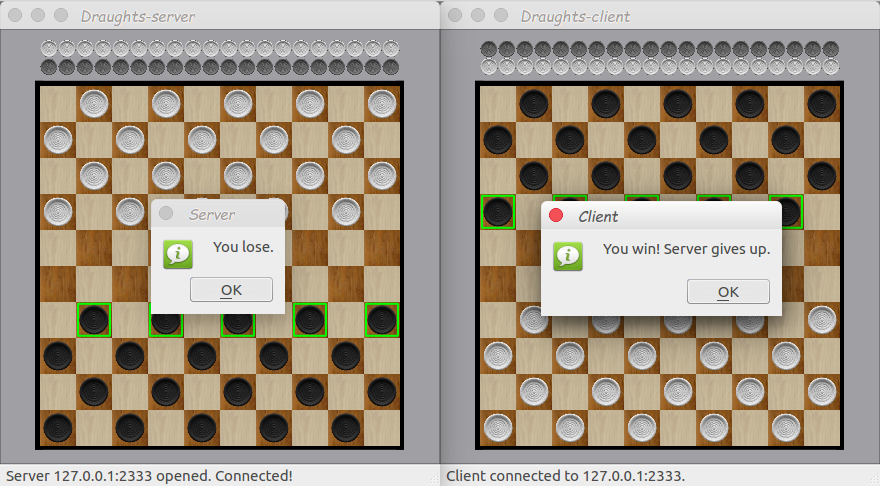
\includegraphics[width=1\linewidth]{giveup.png}
\caption{认输界面}
\label{fig:giveup}
\end{figure}

图~\ref{fig:giveup} 显示了游戏的认输界面,当一方按下Give up选项时,另一方马上会收到请求,游戏立即结束。

\begin{figure}[htbp]
\centering
\subfigure[]
{
\label{fig:draw:a}
\begin{minipage}[b]{0.47\columnwidth}
\centering
\resizebox{\columnwidth}{!}{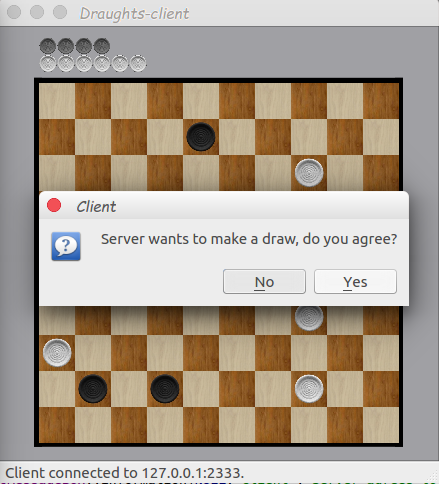
\includegraphics[width=0.5\linewidth]{drawc.png}}
\end{minipage}%
}%
\hfil
\subfigure[]
{
\label{fig:draw:b}
\begin{minipage}[b]{0.47\columnwidth}
\centering
\resizebox{\columnwidth}{!}{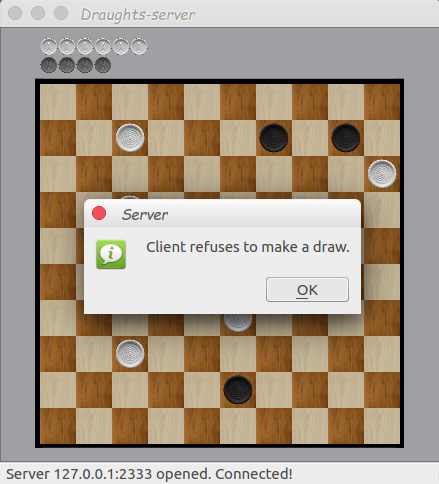
\includegraphics[width=0.5\linewidth]{draws.png}}
\end{minipage}%
}%
\caption{求和界面}\label{fig:draw}
\end{figure}

图~\ref{fig:draw} 显示了求和界面。Server发送求和信息之后,Client需要表态。如果确认求和,那么弹出平局的对话框,游戏结束;如果不同意,那么Server会收到拒绝的信息,此时Client要在40步之内获胜,否则判负。

\section{算法实现}

由于比较懒,只写了一个“上面是白棋,下面是黑棋,黑棋下一步怎么走”的算法核心,使用dfs进行局面的处理。算法核心存储三个$10\times 10$的数组,分别为:局面、可以选的棋子、对于这些可以选的棋子,能够走到哪里(这一步用二进制压位节约空间,因为最多最多只能走20步,一个int有32位)。

每次切换走棋控制权的时候,只需将算法核心中的局面翻转$180^\circ$,并且黑白反色即可。

\section{Qt界面实现}

全部使用QPaintEvent和MousePressEvent进行控制。每次网络传输的时候只传输必要的最少数据:求和请求、认输请求、Input game中的局面字符串,和每次鼠标点击的位置。在数据传输完成之后,由算法核心自动判断当前局面如何进行。

显示的时候,根据当前状态(执黑执白,控制权在哪)将算法核心中的局面映射成用户所希望看到的局面。

至于图片嘛……手动从iPad上面截图修图,[手动微笑]。

代码很丑啊请大佬轻喷qwq
\end{document}